
\begin{frame}{MirageOS}
    
\begin{figure}
    \centering
    \begin{minipage}{0.45\textwidth}
        \centering
        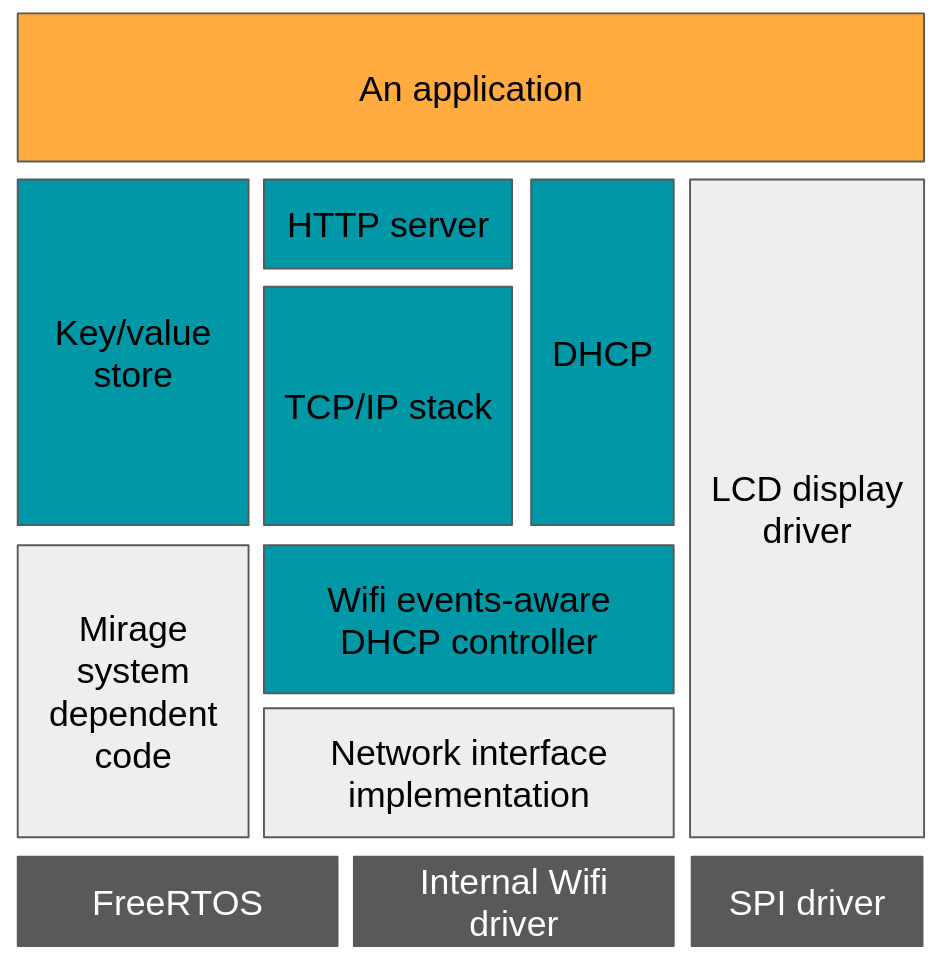
\includegraphics[width=0.9\textwidth]{slides/images/mirage.png}
        \caption{Une application modulaire}
    \end{minipage}\hfill
    \begin{minipage}{0.45\textwidth}
        \centering
        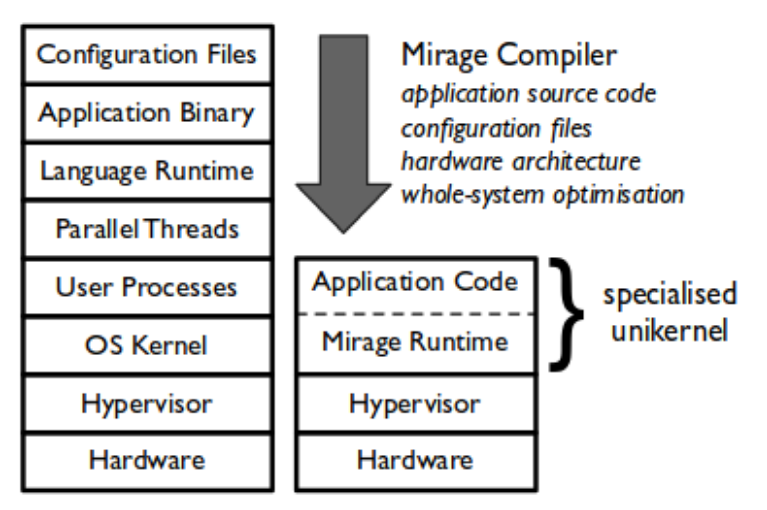
\includegraphics[width=0.9\textwidth]{slides/images/mirage2.png}
        \caption{MirageOS compile à la fois l'application et le système dans un seul exécutable}
    \end{minipage}
\end{figure}

\end{frame}

\begin{frame}[fragile]{Abstraction: signatures de modules}

\begin{lstlisting}
module type Read_only_store = sig 
    type t
    type key = string
    
    val get : t -> key -> string Lwt.t
end
\end{lstlisting}

\begin{lstlisting}
module type HTTP = sig
    type t
    module Request : sig 
        type t
        
        val path : t -> string
    end
    type reponse = string
    
    val listen : t -> (HTTP.Request.t -> response Lwt.t) -> unit Lwt.t
end
\end{lstlisting}


\end{frame}

\begin{frame}[fragile]{Implémentation}
    
\begin{lstlisting}

(* les dependances de notre application sont abstraites 
   via le foncteur Make *)
module Make (FS : Read_only_store) (Server : HTTP) = 
struct
    let start fs http =
        HTTP.listen http (fun request ->
            let path = HTTP.Request.path request in
            FS.get fs path)
end

(* pour les tests *)
module Application = Make (In_memory_store) (Mock_http_server)

(* en production *)
module Application = Make (EXT4) (Cohttp.Server)
\end{lstlisting}

\end{frame}

\begin{frame}{Modules disponibles}
\begin{enumerate}[label=$-$]
    \item Socket réseau: TCP/IP de l'OS ou en OCaml
    \item Stockage: en mémoire, Irmin, FAT
    \item Protocoles: Git, HTTP, SSH, DNS, DHCP
    \item Cryptographie / compression
\end{enumerate}
\end{frame}

%\begin{frame}[fragile]{Boucle d'événements}
%
%\begin{lstlisting}
%val run : unit Lwt.t -> unit
%\end{lstlisting}
%
%\begin{lstlisting}
% let run t =
%   let rec aux () =
%     Time.restart_threads Time.time;
%     match Lwt.poll t with
%     | Some () -> ()
%     | None ->
%         let timeout = Time.select_next () in
%         let ready_set = solo5_yield timeout in
%         (if ready_set <> 0L then
%          (* Some I/O is possible, wake up threads and continue. *)
%          wakeup_threads ready_set);
%         aux ()
%   in
%   aux ()
% \end{lstlisting}
% \end{frame}
